%% ============================================================================
%% Resilient Cognitive Systems - Document
%% Safety-Team 1
%% Authors: Amelie Kleber, Gottlieb Dinh, Jan Chen, Jonathan Deul, Lennard Zei
%% ============================================================================

\documentclass[11pt, a4paper]{article}

%% ============== PACKAGES ==============
\usepackage[utf8]{inputenc}
\usepackage[T1]{fontenc}
\usepackage[margin=2.5cm]{geometry}
\usepackage{fancyhdr}
\usepackage{titlesec}
\usepackage{tocloft}
\usepackage{hyperref}
\usepackage{xcolor}
\usepackage{booktabs}
\usepackage{tabularx}
\usepackage{multirow}
\usepackage{makecell}
\usepackage{colortbl}
\usepackage{array}
\usepackage{longtable}
\usepackage{tikz}
\usepackage{graphicx}
\usepackage{float}
\usepackage{enumitem}
\usepackage{pdflscape}
\usepackage{adjustbox}

%% ============== TIKZ LIBRARIES ==============
\usetikzlibrary{
    shapes.geometric,
    shapes.symbols,
    shapes.misc,
    arrows.meta,
    positioning,
    calc,
    fit,
    backgrounds,
    matrix,
    chains,
    decorations.pathreplacing,
    trees
}

%% ============== COLORS ==============
\definecolor{rcsblue}{HTML}{2B4B6F}
\definecolor{rcsteal}{HTML}{3D8B8B}
\definecolor{rcsgreen}{HTML}{4CAF50}
\definecolor{rcsyellow}{HTML}{F5C242}
\definecolor{rcsorange}{HTML}{E67E22}
\definecolor{rcsred}{HTML}{C0392B}
\definecolor{rcslightblue}{HTML}{5DADE2}
\definecolor{rcsgray}{HTML}{566573}
\definecolor{rcslightgray}{HTML}{F4F6F6}
\definecolor{rcsdarkteal}{HTML}{2C6B6B}

%% ============== HEADER/FOOTER ==============
\pagestyle{fancy}
\fancyhf{}
\fancyhead[L]{\small\textcolor{rcsgray}{Amelie Kleber, Gottlieb Dinh, Jan Chen, Jonathan Deul, Lennard Zei}}
\fancyfoot[C]{\thepage}
\renewcommand{\headrulewidth}{0pt}

%% ============== SECTION STYLING ==============
\titleformat{\section}
    {\color{rcsblue}\Large\bfseries}
    {}{0em}{}
\titleformat{\subsection}
    {\color{rcsblue}\large\bfseries\itshape}
    {}{0em}{}
\titleformat{\subsubsection}
    {\color{rcsteal}\normalsize\bfseries}
    {}{0em}{}

%% ============== TABLE HELPERS ==============
\newcolumntype{H}{>{\columncolor{rcsblue}\color{white}\bfseries}c}
\newcolumntype{G}{>{\columncolor{rcslightgray}}l}
\newcommand{\tableheader}[1]{\cellcolor{rcsblue}\textcolor{white}{\textbf{#1}}}
\newcommand{\rowheader}[1]{\cellcolor{rcslightgray}\textbf{#1}}

%% ============== TIKZ STYLES ==============
\tikzset{
    % Standard filled box
    rcsbox/.style={
        rectangle,
        rounded corners=3pt,
        draw=#1,
        fill=#1,
        text=white,
        font=\small\bfseries,
        minimum height=0.7cm,
        align=center,
        inner sep=4pt
    },
    rcsbox/.default=rcsblue,
    % Outline box
    rcsoutline/.style={
        rectangle,
        rounded corners=2pt,
        draw=#1,
        fill=white,
        text=black,
        font=\small,
        minimum height=0.5cm,
        align=center,
        inner sep=3pt
    },
    rcsoutline/.default=rcsgray,
    % Category header
    categorybox/.style={
        rectangle,
        fill=rcslightgray,
        draw=rcsgray,
        font=\small\bfseries,
        minimum height=0.6cm,
        align=center,
        inner sep=4pt
    },
    % Arrow style
    rcsarrow/.style={
        ->,
        >=Stealth,
        thick,
        color=#1
    },
    rcsarrow/.default=rcsgray,
    % Tree node
    treenode/.style={
        rectangle,
        rounded corners=2pt,
        draw=rcsgray,
        fill=white,
        font=\footnotesize,
        minimum height=0.5cm,
        align=center,
        inner sep=3pt
    },
    % Root node
    rootnode/.style={
        treenode,
        fill=rcsteal,
        text=white,
        font=\footnotesize\bfseries
    },
    % CARE circular node
    carenode/.style={
        circle,
        minimum size=1cm,
        font=\Large\bfseries,
        text=white
    },
    % Process block
    processblock/.style={
        rectangle,
        rounded corners=3pt,
        draw=rcsblue,
        fill=rcsblue,
        text=white,
        font=\small\bfseries,
        minimum height=0.8cm,
        align=center,
        inner sep=4pt
    },
    % Decision diamond
    decisionnode/.style={
        diamond,
        draw=rcsteal,
        fill=rcsteal,
        text=white,
        font=\footnotesize,
        aspect=2,
        inner sep=2pt,
        align=center
    },
    % IO node
    ionode/.style={
        rectangle,
        draw=rcsgray,
        fill=rcslightgray,
        font=\footnotesize,
        minimum height=0.5cm,
        inner sep=3pt
    }
}

%% ============== HYPERREF CONFIG ==============
\hypersetup{
    colorlinks=true,
    linkcolor=rcsblue,
    urlcolor=rcsteal,
    citecolor=rcsgreen
}

%% ============== DOCUMENT ==============
\begin{document}

%% ============== TITLE PAGE ==============
\begin{titlepage}
    \centering
    \vspace*{2cm}

    {\small Amelie Kleber, Gottlieb Dinh, Jan Chen, Jonathan Deul, Lennard Zei}

    \vspace{3cm}

    {\Huge\bfseries\color{rcsblue} Resilient Cognitive Systems -- Document}

    \vspace{1cm}

    {\LARGE Safety-Team 1}

    \vfill
\end{titlepage}

%% ============== TABLE OF CONTENTS ==============
\section*{\color{rcsblue}Contents}
\renewcommand{\contentsname}{}
\vspace{-1cm}
\tableofcontents
\newpage

%% ============== INTRODUCTION ==============
\section{Introduction}

The primary objective of this project is to develop and optimize a safety concept for a robotic arm that interacts with humans in various analysis scenarios. The core challenge lies in ensuring that the robot operates efficiently, while maintaining safety by stopping immediately when a human enters its vicinity.

\subsection*{Project Goals and Constraints}

Following the guidelines of the Resilient Cognitive Systems challenge, we considered the following factors:

\begin{itemize}[leftmargin=*]
    \item \textbf{Safety Criticality:} Any scenario resulting in the robot touching a human leads to a score of zero.
    \item \textbf{Sensor Economy:} While one camera is provided, additional sensors can be integrated at the cost of the overall score.
    \item \textbf{Environmental Adaptability:} The system must remain robust across diverse contexts, including varying light conditions, different human appearances and crowded environments.
    \item \textbf{Infrastructure Limitations:} External safety measures like physical fences or light barriers are strictly prohibited.
\end{itemize}

\subsection*{Methodology}

To ensure a comprehensive safety concept, we employed the following frameworks:

\begin{itemize}[leftmargin=*]
    \item HARA-Analysis
    \item Fault-Tree Analysis
    \item CARE-Analysis
    \item Cause Tree
\end{itemize}

This document details our transition from a vulnerable, camera-only perception system to an improved, multi-sensor architecture designed to provide a high level of efficacy and resilience in human-robot interaction.

\newpage

%% ============== CONTENT ==============
\section{Content}

\subsection{HARA-Analysis}

In order to provide a safety concept with the best possible coverage, we need to clearly define our system, including technical elements and actors involved.

For this, we used the HARA-Analysis introduced in our course. The HARA aims to define the scope of our system and provide a largely complete overview of factors involved by dividing them into 7 steps: The System, Persons at Risk, Hazards \& Hazard types, Physical Properties, Actuator Failure Modes, Actuators and Failure Modes.

From there on, we used these categories to combine them into HARA-guide phrases to serve as exemplary hazard cases to countermeasure against.

To provide a proof of completeness for the HARA-analysis, we opted for a traceability matrix (Figure 1) that compares Physical Properties against all other HARA-categories, except for the actuators. The reason for this selection was that we were sure of the completeness of the two actuators in our system. Each Physical property could be traced back to one of the actuators that it affected and was therefore more likely to be complete as well. Reading the matrix from left to right provides the remaining guide-phrases.

%% Figure 1: HARA Categories
\begin{figure}[H]
\centering
\begin{tikzpicture}[node distance=0.15cm, scale=0.85, transform shape]

    % Column 1: System
    \node[categorybox, text width=2.5cm] (sys-header) {System};
    \node[rcsoutline, below=of sys-header, text width=2.5cm, minimum height=1.5cm] (sys-item) {
        A robot arm with\\pick and place\\functionality
    };

    % Column 2: Persons at Risk
    \node[categorybox, right=0.3cm of sys-header, text width=2.2cm] (por-header) {Persons at Risk};
    \node[rcsoutline, below=of por-header, text width=2.2cm] (por-tech) {Technician};
    \node[rcsoutline, below=0.1cm of por-tech, text width=2.2cm] (por-op) {Operator};

    % Column 3: Physical Properties
    \node[categorybox, right=0.3cm of por-header, text width=2.2cm] (pp-header) {Physical Properties};
    \node[rcsoutline, below=of pp-header, text width=2.2cm] (pp1) {Voltage};
    \node[rcsoutline, below=0.1cm of pp1, text width=2.2cm] (pp2) {Program};
    \node[rcsoutline, below=0.1cm of pp2, text width=2.2cm] (pp3) {Weight of Cargo};
    \node[rcsoutline, below=0.1cm of pp3, text width=2.2cm] (pp4) {(Position, Velocity)};

    % Column 4: Actuator Failure Modes
    \node[categorybox, right=0.3cm of pp-header, text width=2.4cm] (afm-header) {Actuator Failure\\Modes};
    \node[rcsoutline, below=of afm-header, text width=2.4cm, minimum height=1cm] (afm1) {Provision\\Commission};
    \node[rcsoutline, below=0.1cm of afm1, text width=2.4cm, minimum height=1cm] (afm2) {Data Coarse\\Incorrect};

    % Column 5: Actuators
    \node[categorybox, right=0.3cm of afm-header, text width=1.8cm] (act-header) {Actuators};
    \node[rcsoutline, below=of act-header, text width=1.8cm] (act1) {Battery};
    \node[rcsoutline, below=0.1cm of act1, text width=1.8cm] (act2) {Motors};

    % Hazards section (below System)
    \node[categorybox, below=0.8cm of sys-item, text width=2.5cm] (haz-header) {Hazards};

    % Mechanical hazards row
    \node[below=0.15cm of haz-header.south west, anchor=north west] (mech-row) {
        \begin{tikzpicture}[node distance=0.1cm]
            \node[circle, fill=rcsblue, minimum size=0.35cm, inner sep=0pt] (mech-icon) {};
            \node[font=\scriptsize, right=0.1cm of mech-icon] {Mechanical};
            \node[rcsoutline, right=0.15cm of previous, text width=1.6cm, font=\scriptsize] (coll-robot) {Collision with Robot};
            \node[rcsoutline, right=0.1cm of coll-robot, text width=1.6cm, font=\scriptsize] {Collision with Cargo};
        \end{tikzpicture}
    };

    % Electrical hazards row
    \node[below=0.1cm of mech-row.south west, anchor=north west] (elec-row) {
        \begin{tikzpicture}[node distance=0.1cm]
            \node[regular polygon, regular polygon sides=3, fill=rcsyellow, minimum size=0.4cm, inner sep=0pt] (elec-icon) {};
            \node[font=\scriptsize, right=0.1cm of elec-icon] {Electrical};
            \node[rcsoutline, right=0.15cm of previous, text width=2cm, font=\scriptsize] {Electric Shock};
        \end{tikzpicture}
    };

    % Thermal hazards row
    \node[below=0.1cm of elec-row.south west, anchor=north west] (therm-row) {
        \begin{tikzpicture}[node distance=0.1cm]
            \node[circle, fill=rcsorange, minimum size=0.35cm, inner sep=0pt] (therm-icon) {};
            \node[font=\scriptsize, right=0.1cm of therm-icon] {Thermal};
            \node[rcsoutline, right=0.15cm of previous, text width=2cm, font=\scriptsize] {Ignition Hazard};
        \end{tikzpicture}
    };

    % Failure Modes (right side)
    \node[categorybox, right=0.3cm of act-header, text width=2.2cm] (fm-header) {Failure Modes};
    \node[rcsoutline, below=of fm-header, text width=2.2cm, font=\scriptsize] (fm1) {Arm moves into person};
    \node[rcsoutline, below=0.1cm of fm1, text width=2.2cm, font=\scriptsize] (fm2) {Arm drops Cargo onto person};
    \node[rcsoutline, below=0.1cm of fm2, text width=2.2cm, font=\scriptsize] (fm3) {Arm electrocutes person};
    \node[rcsoutline, below=0.1cm of fm3, text width=2.2cm, font=\scriptsize] (fm4) {Arm causes Ignition};

\end{tikzpicture}
\caption{HARA System Definition Categories}
\label{fig:hara-categories}
\end{figure}

%% Figure 2: Guide Phrases
\begin{figure}[H]
\centering
\begin{tikzpicture}[node distance=0.3cm, scale=0.9, transform shape]

    % Guide phrase question box (left side)
    \node[rcsoutline=rcsgray, text width=5.5cm, minimum height=2.5cm, align=left, inner sep=8pt] (question) {
        Could a \textcolor{rcsred}{\textbf{failure mode}} of an \textcolor{rcsblue}{\textbf{actuator}} cause an unintended impact on the \textcolor{rcsteal}{\textbf{physical property}} causing a \textcolor{rcsorange}{\textbf{hazard}}?
    };

    % Box 1 (top right)
    \node[right=1.2cm of question, yshift=1.8cm] (box1) {
        \begin{tikzpicture}[node distance=0.08cm]
            \node[font=\scriptsize\bfseries, fill=rcsblue, text=white, inner sep=2pt] (num1) {1.};
            \node[rcsbox=rcsblue, right=0.1cm of num1, text width=2.3cm, font=\scriptsize\bfseries] (b1-fm) {Arm moves into person};
            \node[rcsbox=rcsgreen, right=0.08cm of b1-fm, text width=1.3cm, font=\scriptsize\bfseries] (b1-act) {Motors};

            \node[rcsbox=rcsteal, below=0.15cm of b1-fm.south west, anchor=north west, text width=1.5cm, font=\scriptsize\bfseries] (b1-afm) {Data coarse incorrect};
            \node[rcsbox=rcsteal, right=0.08cm of b1-afm, text width=1.5cm, font=\scriptsize\bfseries] (b1-pp) {(Position, Velocity)};
            \node[rcsbox=rcsorange, right=0.08cm of b1-pp, text width=1.5cm, font=\scriptsize\bfseries] (b1-haz) {Collision with Robot};
        \end{tikzpicture}
    };

    % Box 2 (middle right)
    \node[right=1.2cm of question, yshift=-0.3cm] (box2) {
        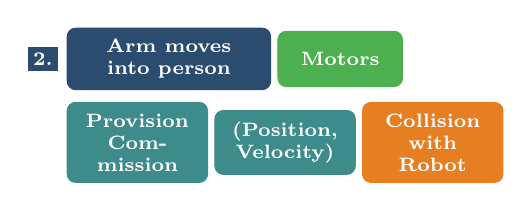
\begin{tikzpicture}[node distance=0.08cm]
            \node[font=\scriptsize\bfseries, fill=rcsblue, text=white, inner sep=2pt] (num2) {2.};
            \node[rcsbox=rcsblue, right=0.1cm of num2, text width=2.3cm, font=\scriptsize\bfseries] (b2-fm) {Arm moves into person};
            \node[rcsbox=rcsgreen, right=0.08cm of b2-fm, text width=1.3cm, font=\scriptsize\bfseries] (b2-act) {Motors};

            \node[rcsbox=rcsteal, below=0.15cm of b2-fm.south west, anchor=north west, text width=1.5cm, font=\scriptsize\bfseries] (b2-afm) {Provision Commission};
            \node[rcsbox=rcsteal, right=0.08cm of b2-afm, text width=1.5cm, font=\scriptsize\bfseries] (b2-pp) {(Position, Velocity)};
            \node[rcsbox=rcsorange, right=0.08cm of b2-pp, text width=1.5cm, font=\scriptsize\bfseries] (b2-haz) {Collision with Robot};
        \end{tikzpicture}
    };

    % Box 3 (bottom right)
    \node[right=1.2cm of question, yshift=-2.4cm] (box3) {
        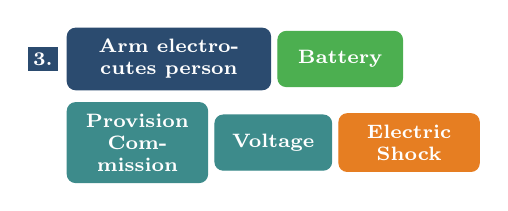
\begin{tikzpicture}[node distance=0.08cm]
            \node[font=\scriptsize\bfseries, fill=rcsblue, text=white, inner sep=2pt] (num3) {3.};
            \node[rcsbox=rcsblue, right=0.1cm of num3, text width=2.3cm, font=\scriptsize\bfseries] (b3-fm) {Arm electrocutes person};
            \node[rcsbox=rcsgreen, right=0.08cm of b3-fm, text width=1.3cm, font=\scriptsize\bfseries] (b3-act) {Battery};

            \node[rcsbox=rcsteal, below=0.15cm of b3-fm.south west, anchor=north west, text width=1.5cm, font=\scriptsize\bfseries] (b3-afm) {Provision Commission};
            \node[rcsbox=rcsteal, right=0.08cm of b3-afm, text width=1.2cm, font=\scriptsize\bfseries] (b3-pp) {Voltage};
            \node[rcsbox=rcsorange, right=0.08cm of b3-pp, text width=1.5cm, font=\scriptsize\bfseries] (b3-haz) {Electric Shock};
        \end{tikzpicture}
    };

\end{tikzpicture}
\caption{HARA Guide Phrases}
\label{fig:hara-guide-phrases}
\end{figure}

\newpage

\subsection{Previous System Architecture}

We define the robotic arm system in detail using a three-level architecture that takes in the arm's current position and the desired movement plan.

In the first level, we discern several elements:
\begin{itemize}[leftmargin=*]
    \item \textbf{Mission planner}, which receives a mission and outputs a target and object
    \item \textbf{Obstacle Detection}, which receives camera information and outputs an object list
    \item \textbf{Gripper Sensor}, which receives the grip strength and grip width and outputs the grip percentage and strength
    \item \textbf{Joint Motor Sensors}, which receive the position, velocity, and acceleration of the joint motors and output a vector consisting of the three numbers
\end{itemize}

At the second level, the \textbf{Trajectory Planner} receives the outputs and maps them to a trajectory consisting of the arm's current and next positions. Additionally, it outputs the time to destination.

The third level \textbf{Trajectory Control} transforms them into six different degrees for each joint motor of the robot arm, with one additional vector for the robot grip. This represents the actual movement of the arm to fulfil the mission.

%% Figure 3: System Architecture
\begin{figure}[H]
\centering
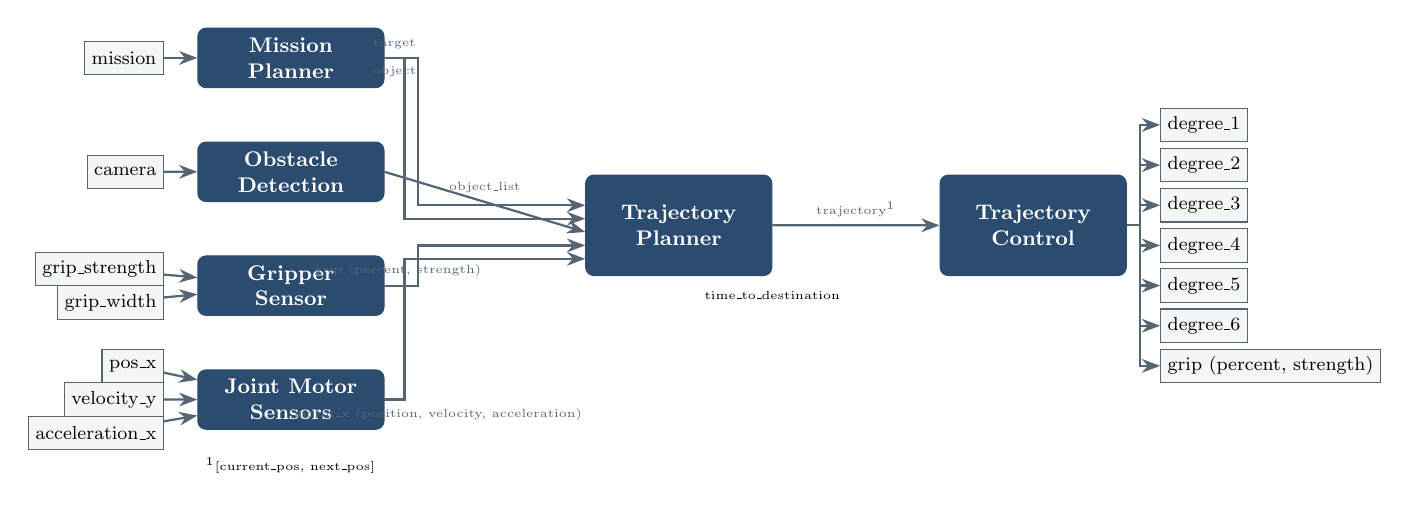
\begin{tikzpicture}[node distance=0.6cm, scale=0.85, transform shape]

    % Level 1 blocks (left side)
    \node[processblock, text width=2.5cm] (mission) {Mission Planner};
    \node[processblock, text width=2.5cm, below=0.8cm of mission] (obstacle) {Obstacle\\Detection};
    \node[processblock, text width=2.5cm, below=0.8cm of obstacle] (gripper) {Gripper Sensor};
    \node[processblock, text width=2.5cm, below=0.8cm of gripper] (joint) {Joint Motor\\Sensors};

    % Input labels (left of level 1)
    \node[ionode, left=0.5cm of mission] (in-mission) {\footnotesize mission};
    \node[ionode, left=0.5cm of obstacle] (in-camera) {\footnotesize camera};
    \node[ionode, left=0.5cm of gripper, yshift=0.25cm] (in-grip-str) {\footnotesize grip\_strength};
    \node[ionode, left=0.5cm of gripper, yshift=-0.25cm] (in-grip-wid) {\footnotesize grip\_width};
    \node[ionode, left=0.5cm of joint, yshift=0.5cm] (in-pos) {\footnotesize pos\_x};
    \node[ionode, left=0.5cm of joint] (in-vel) {\footnotesize velocity\_y};
    \node[ionode, left=0.5cm of joint, yshift=-0.5cm] (in-acc) {\footnotesize acceleration\_x};

    % Level 2 block (middle)
    \node[processblock, text width=2.5cm, minimum height=1.5cm, right=3cm of obstacle, yshift=-0.8cm] (traj-plan) {Trajectory\\Planner};

    % Level 3 block (right)
    \node[processblock, text width=2.5cm, minimum height=1.5cm, right=2.5cm of traj-plan] (traj-ctrl) {Trajectory\\Control};

    % Output labels (right of level 3)
    \node[ionode, right=0.5cm of traj-ctrl, yshift=1.5cm] (out-deg1) {\footnotesize degree\_1};
    \node[ionode, right=0.5cm of traj-ctrl, yshift=0.9cm] (out-deg2) {\footnotesize degree\_2};
    \node[ionode, right=0.5cm of traj-ctrl, yshift=0.3cm] (out-deg3) {\footnotesize degree\_3};
    \node[ionode, right=0.5cm of traj-ctrl, yshift=-0.3cm] (out-deg4) {\footnotesize degree\_4};
    \node[ionode, right=0.5cm of traj-ctrl, yshift=-0.9cm] (out-deg5) {\footnotesize degree\_5};
    \node[ionode, right=0.5cm of traj-ctrl, yshift=-1.5cm] (out-deg6) {\footnotesize degree\_6};
    \node[ionode, right=0.5cm of traj-ctrl, yshift=-2.1cm] (out-grip) {\footnotesize grip (percent, strength)};

    % Input arrows
    \draw[rcsarrow] (in-mission) -- (mission);
    \draw[rcsarrow] (in-camera) -- (obstacle);
    \draw[rcsarrow] (in-grip-str) -- (gripper);
    \draw[rcsarrow] (in-grip-wid) -- (gripper);
    \draw[rcsarrow] (in-pos) -- (joint);
    \draw[rcsarrow] (in-vel) -- (joint);
    \draw[rcsarrow] (in-acc) -- (joint);

    % Intermediate connections with labels
    \draw[rcsarrow] (mission.east) -- ++(0.5,0) node[above, font=\tiny, pos=0.3] {target} |- ([yshift=0.3cm]traj-plan.west);
    \draw[rcsarrow] (mission.east) -- ++(0.3,0) node[below, font=\tiny, pos=0.5] {object} |- ([yshift=0.1cm]traj-plan.west);
    \draw[rcsarrow] (obstacle.east) -- node[above, font=\tiny] {object\_list} ([yshift=-0.1cm]traj-plan.west);
    \draw[rcsarrow] (gripper.east) -- ++(0.5,0) node[above, font=\tiny, xshift=-0.3cm] {grip (percent, strength)} |- ([yshift=-0.3cm]traj-plan.west);
    \draw[rcsarrow] (joint.east) -- ++(0.3,0) node[below, font=\tiny, xshift=0.5cm] {motor\_x (position, velocity, acceleration)} |- ([yshift=-0.5cm]traj-plan.west);

    % Trajectory planner to control
    \draw[rcsarrow] (traj-plan.east) -- node[above, font=\tiny] {trajectory\textsuperscript{1}} (traj-ctrl.west);
    \node[below=0.1cm of traj-plan.south east, font=\tiny, anchor=north] {time\_to\_destination};

    % Output arrows
    \draw[rcsarrow] (traj-ctrl.east) -- ++(0.2,0) |- (out-deg1);
    \draw[rcsarrow] (traj-ctrl.east) -- ++(0.2,0) |- (out-deg2);
    \draw[rcsarrow] (traj-ctrl.east) -- ++(0.2,0) |- (out-deg3);
    \draw[rcsarrow] (traj-ctrl.east) -- ++(0.2,0) |- (out-deg4);
    \draw[rcsarrow] (traj-ctrl.east) -- ++(0.2,0) |- (out-deg5);
    \draw[rcsarrow] (traj-ctrl.east) -- ++(0.2,0) |- (out-deg6);
    \draw[rcsarrow] (traj-ctrl.east) -- ++(0.2,0) |- (out-grip);

    % Footnote
    \node[below=0.3cm of joint.south west, anchor=north west, font=\tiny] {\textsuperscript{1}[current\_pos, next\_pos]};

\end{tikzpicture}
\caption{Previous System Architecture}
\label{fig:prev-architecture}
\end{figure}

\newpage

\subsection{Limitations with Previous System Architecture}

However, camera-only perception cannot guarantee safe human detection due to variable visibility, signal degradation, and ambiguous interpretation by ML models. We defined three broad categories for limitations imposed on our previous System Architecture.

%% Figure 4: Limitations
\begin{figure}[H]
\centering
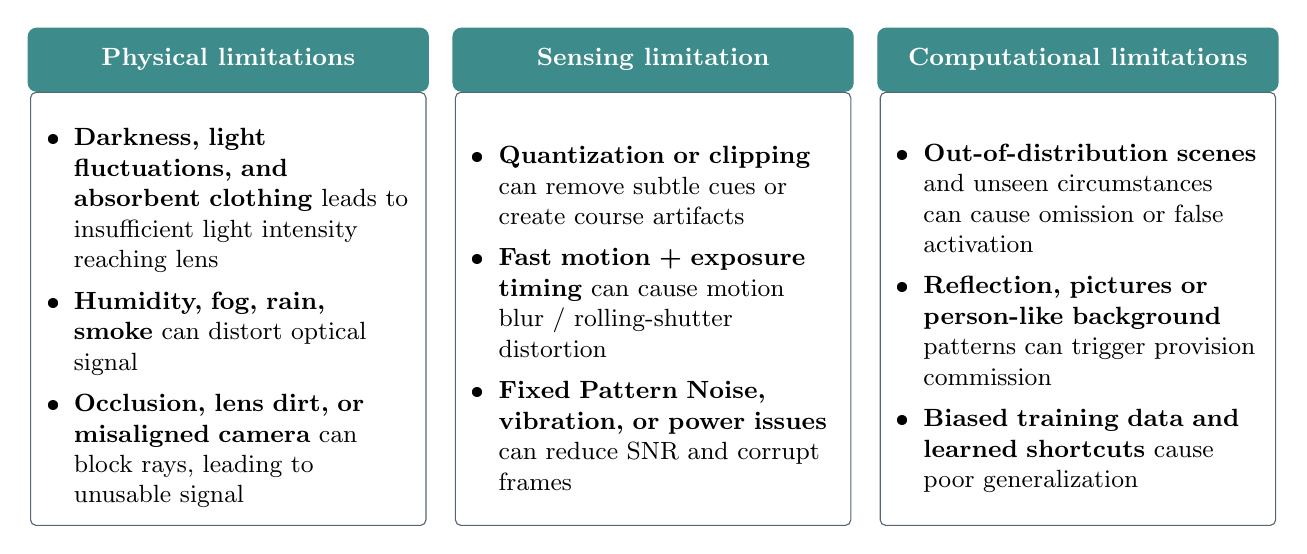
\begin{tikzpicture}[node distance=0.2cm]

    % Headers
    \node[rcsbox=rcsteal, text width=4.8cm, minimum height=0.8cm] (h1) {Physical limitations};
    \node[rcsbox=rcsteal, text width=4.8cm, minimum height=0.8cm, right=0.3cm of h1] (h2) {Sensing limitation};
    \node[rcsbox=rcsteal, text width=4.8cm, minimum height=0.8cm, right=0.3cm of h2] (h3) {Computational limitations};

    % Content boxes
    \node[rcsoutline=rcsgray, text width=4.6cm, minimum height=5.5cm, below=0cm of h1, align=left, inner sep=6pt] (c1) {
        \begin{itemize}[leftmargin=*, itemsep=4pt, parsep=0pt, topsep=2pt]
            \item \textbf{Darkness, light fluctuations, and absorbent clothing} leads to insufficient light intensity reaching lens
            \item \textbf{Humidity, fog, rain, smoke} can distort optical signal
            \item \textbf{Occlusion, lens dirt, or misaligned camera} can block rays, leading to unusable signal
        \end{itemize}
    };

    \node[rcsoutline=rcsgray, text width=4.6cm, minimum height=5.5cm, below=0cm of h2, align=left, inner sep=6pt] (c2) {
        \begin{itemize}[leftmargin=*, itemsep=4pt, parsep=0pt, topsep=2pt]
            \item \textbf{Quantization or clipping} can remove subtle cues or create course artifacts
            \item \textbf{Fast motion + exposure timing} can cause motion blur / rolling-shutter distortion
            \item \textbf{Fixed Pattern Noise, vibration, or power issues} can reduce SNR and corrupt frames
        \end{itemize}
    };

    \node[rcsoutline=rcsgray, text width=4.6cm, minimum height=5.5cm, below=0cm of h3, align=left, inner sep=6pt] (c3) {
        \begin{itemize}[leftmargin=*, itemsep=4pt, parsep=0pt, topsep=2pt]
            \item \textbf{Out-of-distribution scenes} and unseen circumstances can cause omission or false activation
            \item \textbf{Reflection, pictures or person-like background} patterns can trigger provision commission
            \item \textbf{Biased training data and learned shortcuts} cause poor generalization
        \end{itemize}
    };

\end{tikzpicture}
\caption{Limitations with Previous System Architecture}
\label{fig:limitations}
\end{figure}

\subsection{Fault-Tree Analysis - Gottlieb}

We analysed the architecture level by level to identify every possible fault. For this we defined our top fault ``robot arm moves even though it should not'' as degree of motor x is too high.

%% Figure 5: Fault Tree
\begin{figure}[H]
\centering
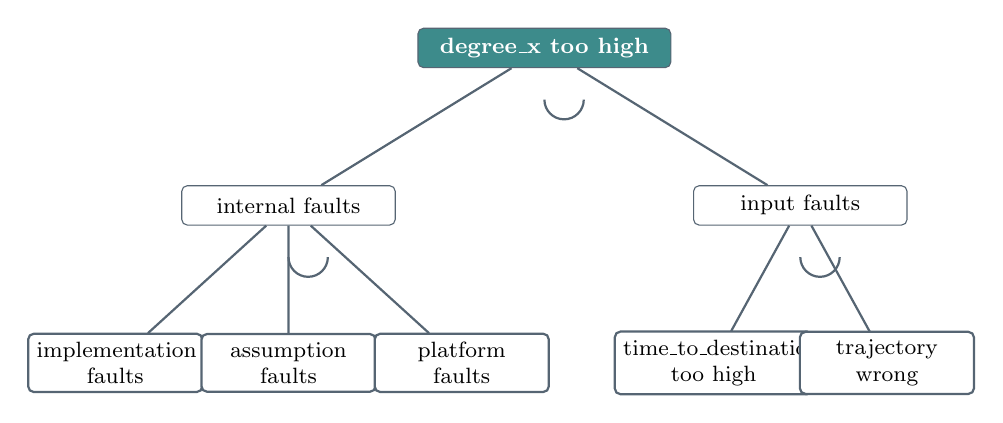
\begin{tikzpicture}[
    level 1/.style={sibling distance=6.5cm, level distance=2cm},
    level 2/.style={sibling distance=2.2cm, level distance=2cm},
    edge from parent/.style={draw, thick, rcsgray},
    every node/.style={align=center}
]

    % Root node
    \node[rootnode, text width=3cm] (root) {degree\_x too high}
        child {
            node[treenode, text width=2.5cm] (internal) {internal faults}
            child {node[treenode, text width=2cm] {implementation\\faults}}
            child {node[treenode, text width=2cm] {assumption\\faults}}
            child {node[treenode, text width=2cm] {platform\\faults}}
        }
        child {
            node[treenode, text width=2.5cm] (input) {input faults}
            child {node[treenode, text width=2.3cm] {time\_to\_destination\\too high}}
            child {node[treenode, text width=2cm] {trajectory\\wrong}}
        };

    % OR gate symbols (arcs below nodes)
    \draw[thick, rcsgray] ([yshift=-0.4cm]root.south) arc (180:360:0.25cm);
    \draw[thick, rcsgray] ([yshift=-0.4cm]internal.south) arc (180:360:0.25cm);
    \draw[thick, rcsgray] ([yshift=-0.4cm]input.south) arc (180:360:0.25cm);

\end{tikzpicture}
\caption{Fault-Tree Analysis}
\label{fig:fault-tree}
\end{figure}

\newpage

\subsection{CARE-Analysis}

CARE adds structure for perception and actuation analysis by subdividing it into single steps that provide a basis for systematic analysis and coverage. In the following, we will focus only on the sense half of the model, as our system is detection-oriented. The analysis is subdivided into four steps. Each step provides a source, a model, the model's assumptions, a sink, an insufficiency backlog, and some exemplary analysis cases. For completeness, each step is accompanied by a traceability matrix that matches Assumptions to Failure Modes.

\begin{itemize}[leftmargin=*]
    \item \textbf{C->A:} We examine insufficiencies that might occur and lead to differences between the actual value and the sensed value, causing erroneous detection. (Figure 2 + 3 in Appendix)
    \item \textbf{A->R:} We examine insufficiencies that might occur and lead to differences between the actually sensed value and the digital representation of the value, causing erroneous detection. (Figure 4 + 5 in Appendix)
    \item \textbf{R->E:} We examine insufficiencies that might occur and lead to differences between the digital representation of the value and the estimated value, causing erroneous detection. (Figure 6+7 in Appendix)
\end{itemize}

%% Figure 6: CARE Model
\begin{figure}[H]
\centering
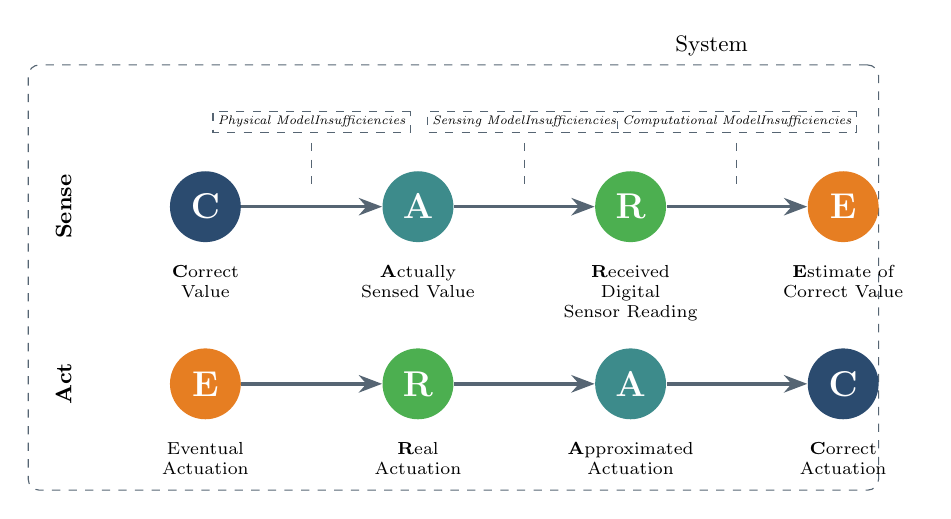
\begin{tikzpicture}[node distance=0.5cm, scale=0.9, transform shape]

    % System boundary box (dashed)
    \node[draw=rcsgray, dashed, rounded corners, minimum width=12cm, minimum height=6cm, label={[font=\small]above right:System}] (system) {};

    % SENSE row label
    \node[font=\small\bfseries, rotate=90] at (-5.5, 1) {Sense};

    % SENSE row nodes
    \node[carenode, fill=rcsblue] (C1) at (-3.5, 1) {C};
    \node[carenode, fill=rcsteal] (A1) at (-0.5, 1) {A};
    \node[carenode, fill=rcsgreen] (R1) at (2.5, 1) {R};
    \node[carenode, fill=rcsorange] (E1) at (5.5, 1) {E};

    % SENSE labels
    \node[font=\scriptsize, below=0.2cm of C1, text width=1.8cm, align=center] {\textbf{C}orrect\\Value};
    \node[font=\scriptsize, below=0.2cm of A1, text width=1.8cm, align=center] {\textbf{A}ctually\\Sensed Value};
    \node[font=\scriptsize, below=0.2cm of R1, text width=2cm, align=center] {\textbf{R}eceived Digital\\Sensor Reading};
    \node[font=\scriptsize, below=0.2cm of E1, text width=2cm, align=center] {\textbf{E}stimate of\\Correct Value};

    % SENSE arrows
    \draw[rcsarrow=rcsgray, very thick] (C1) -- (A1);
    \draw[rcsarrow=rcsgray, very thick] (A1) -- (R1);
    \draw[rcsarrow=rcsgray, very thick] (R1) -- (E1);

    % Insufficiency labels (above arrows)
    \node[draw=rcsgray, dashed, font=\tiny\itshape, inner sep=2pt, fill=white] at (-2, 2.2) {Physical Model\\Insufficiencies};
    \node[draw=rcsgray, dashed, font=\tiny\itshape, inner sep=2pt, fill=white] at (1, 2.2) {Sensing Model\\Insufficiencies};
    \node[draw=rcsgray, dashed, font=\tiny\itshape, inner sep=2pt, fill=white] at (4, 2.2) {Computational Model\\Insufficiencies};

    % Dashed lines to arrows
    \draw[dashed, rcsgray] (-2, 1.9) -- (-2, 1.3);
    \draw[dashed, rcsgray] (1, 1.9) -- (1, 1.3);
    \draw[dashed, rcsgray] (4, 1.9) -- (4, 1.3);

    % ACT row label
    \node[font=\small\bfseries, rotate=90] at (-5.5, -1.5) {Act};

    % ACT row nodes
    \node[carenode, fill=rcsorange] (E2) at (-3.5, -1.5) {E};
    \node[carenode, fill=rcsgreen] (R2) at (-0.5, -1.5) {R};
    \node[carenode, fill=rcsteal] (A2) at (2.5, -1.5) {A};
    \node[carenode, fill=rcsblue] (C2) at (5.5, -1.5) {C};

    % ACT labels
    \node[font=\scriptsize, below=0.2cm of E2, text width=1.8cm, align=center] {Eventual\\Actuation};
    \node[font=\scriptsize, below=0.2cm of R2, text width=1.8cm, align=center] {\textbf{R}eal\\Actuation};
    \node[font=\scriptsize, below=0.2cm of A2, text width=2cm, align=center] {\textbf{A}pproximated\\Actuation};
    \node[font=\scriptsize, below=0.2cm of C2, text width=1.8cm, align=center] {\textbf{C}orrect\\Actuation};

    % ACT arrows (reversed direction)
    \draw[rcsarrow=rcsgray, very thick] (E2) -- (R2);
    \draw[rcsarrow=rcsgray, very thick] (R2) -- (A2);
    \draw[rcsarrow=rcsgray, very thick] (A2) -- (C2);

\end{tikzpicture}
\caption{CARE Analysis Model}
\label{fig:care-model}
\end{figure}

\newpage

\subsection{Cause Tree -- Jan}

Based on the results of the HARA, fault-tree, and CARE analyses, we derive a cause tree to systematically explain how a person in the hazard zone may remain undetected.

At the highest level, the unwanted event can occur either because a valid image is available but misinterpreted by the computational model, or because the image is already insufficient at the model input. These two branches directly map to the CARE structure. Computational model insufficiencies occur during the R$\rightarrow$E step and include cases in which available digital data is incorrectly interpreted due to biased or insufficient training data, limited model capacity, or inappropriate runtime thresholds and decision logic.

In contrast, insufficient model input is further decomposed into sensing and physical model insufficiencies. Sensing model insufficiencies correspond to the A$\rightarrow$R step and describe failures in sensing and digitization, such as limited dynamic range or quantization, inadequate temporal sampling or exposure, sensor noise, spectral mismatch, or preprocessing that removes relevant details. Physical model insufficiencies reflect the C$\rightarrow$A step and describe violations of real-world assumptions at the optical input, for example, due to unfavorable lighting, unexpected appearance or reflectance of a person, environmental influences on light propagation, or geometric constraints such as occlusion or a limited field of view. The cause tree highlights recurring insufficiencies across the CARE layers, which directly define the points addressed by the proposed safety concept.

%% Figure 7: Cause Tree
\begin{figure}[H]
\centering
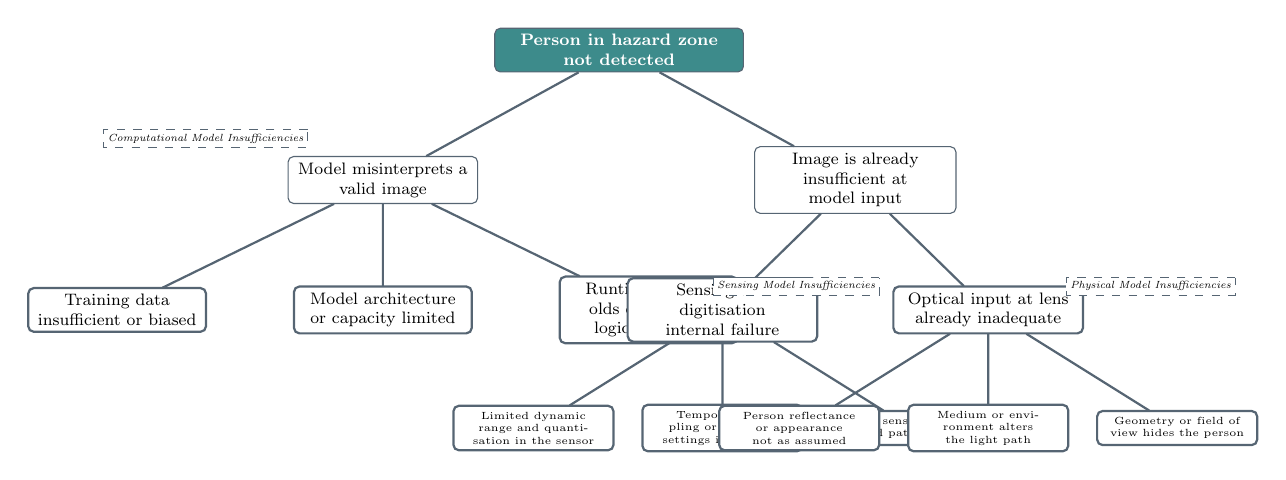
\begin{tikzpicture}[
    scale=0.75, transform shape,
    level 1/.style={sibling distance=8cm, level distance=2.2cm},
    level 2/.style={sibling distance=4.5cm, level distance=2.2cm},
    level 3/.style={sibling distance=3.2cm, level distance=2cm},
    edge from parent/.style={draw, thick, rcsgray},
    every node/.style={align=center}
]

    % Root
    \node[rootnode, text width=4cm] (root) {Person in hazard zone\\not detected}
        child {
            node[treenode, text width=3cm] (model-mis) {Model misinterprets a\\valid image}
            child {node[treenode, text width=2.8cm] {Training data insufficient or biased}}
            child {node[treenode, text width=2.8cm] {Model architecture or capacity limited}}
            child {node[treenode, text width=2.8cm] {Runtime thresholds or decision logic incorrect}}
        }
        child {
            node[treenode, text width=3.2cm] (image-insuff) {Image is already\\insufficient at model input}
            child {
                node[treenode, text width=3cm] (sensing) {Sensing and digitisation\\internal failure}
                child {node[treenode, text width=2.5cm, font=\tiny] {Limited dynamic range and quantisation in the sensor}}
                child {node[treenode, text width=2.5cm, font=\tiny] {Temporal sampling or exposure settings inadequate}}
                child {node[treenode, text width=2.5cm, font=\tiny] {High sensor noise or fixed pattern noise}}
            }
            child {
                node[treenode, text width=3cm] (optical) {Optical input at lens\\already inadequate}
                child {node[treenode, text width=2.5cm, font=\tiny] {Person reflectance or appearance not as assumed}}
                child {node[treenode, text width=2.5cm, font=\tiny] {Medium or environment alters the light path}}
                child {node[treenode, text width=2.5cm, font=\tiny] {Geometry or field of view hides the person}}
            }
        };

    % Category labels
    \node[draw=rcsgray, dashed, font=\tiny\itshape, fill=white, inner sep=2pt] at (-7, -1.5) {Computational Model Insufficiencies};
    \node[draw=rcsgray, dashed, font=\tiny\itshape, fill=white, inner sep=2pt] at (3, -4) {Sensing Model Insufficiencies};
    \node[draw=rcsgray, dashed, font=\tiny\itshape, fill=white, inner sep=2pt] at (9, -4) {Physical Model Insufficiencies};

\end{tikzpicture}
\caption{Cause Tree}
\label{fig:cause-tree}
\end{figure}

\newpage

\subsection{Improved Safety Concept - Lennard}

To move away from our previous Safety Concept/Architecture, which relied solely on camera vision and had severe limitations, we opted for a dual-sensor setup. In addition to the optical camera data, the Object Detection element receives readings from a mmWave sensor. Depending on the readings, it either outputs an empty object list, indicating it will not stop, or an array containing the position of the detected movement, leading it to stop all movement.

When the mmWave detects movement = false, it outputs an empty array directly to the object list. If detects movement = true, we determine how far away the movement is. If it is greater than 2 meters away we once again pass on an empty array list, since the object is too far away to stop. If it closer than 2 meters we pass on an array with the position of all movement.

In the next step, we determine whether the detected movement was from a robot or not. For that we use the optical data from the camera. In order for a robot to be identified we use both a QR-Code for detection and a Classification trained on recognizing robots. If both these measures are true, an empty array list is passed to the Object list, since we do not want to stop when robots interact with each other. However, if only one of these measure returns false, we decide that a non-human entity is detected and we stop just in case by passing the position of all movement to the Object List.

\subsection{CARE Analysis of Improved Safety Concept - Gottlieb}

\subsection{Evidence of Efficacy -- Gottlieb}

%% Figure 8: Improved Safety Concept
\begin{figure}[H]
\centering
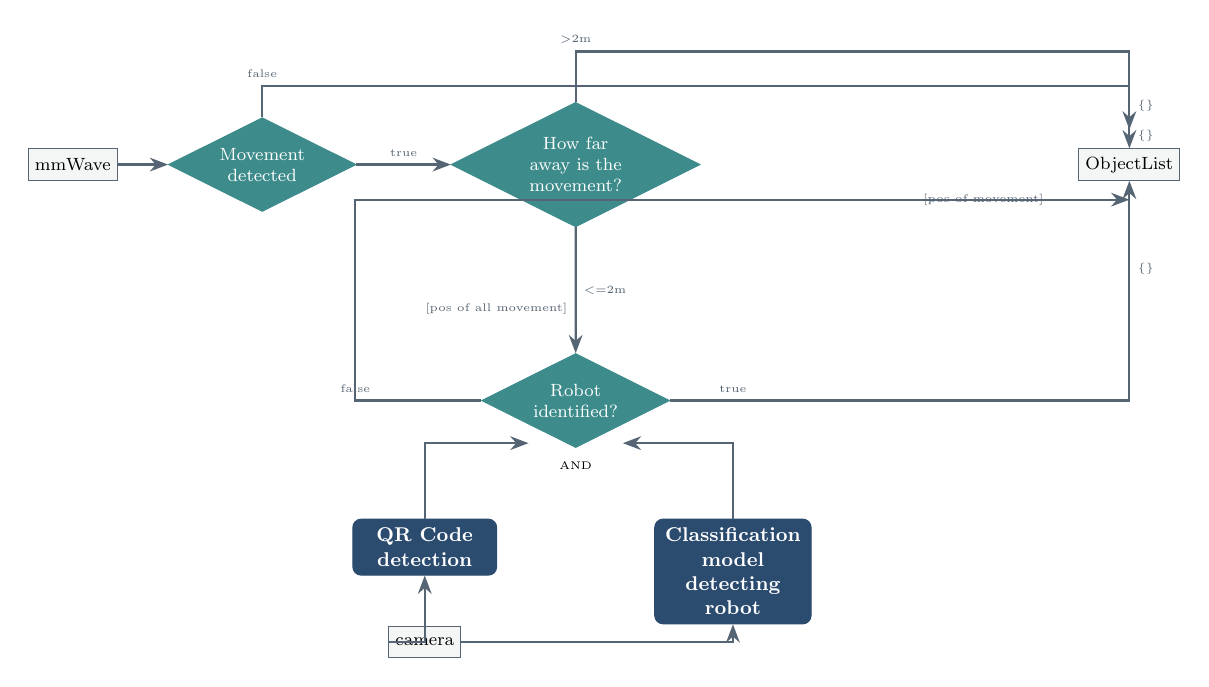
\begin{tikzpicture}[node distance=0.6cm, scale=0.8, transform shape]

    % mmWave input
    \node[ionode] (mmwave) {mmWave};

    % Movement detected decision
    \node[decisionnode, right=0.8cm of mmwave, text width=1.5cm] (detect) {Movement\\detected};

    % Distance decision
    \node[decisionnode, right=1.5cm of detect, text width=1.8cm] (distance) {How far away is the movement?};

    % Object List output
    \node[ionode, right=6cm of distance] (objlist) {Object\\List};

    % Robot identified decision
    \node[decisionnode, below=2cm of distance, text width=1.5cm] (robot) {Robot\\identified?};

    % QR Code detection
    \node[processblock, below left=1.5cm and 0.5cm of robot, text width=2cm] (qr) {QR Code\\detection};

    % Classification model
    \node[processblock, below right=1.5cm and 0.5cm of robot, text width=2.2cm] (classify) {Classification model\\detecting robot};

    % Camera input
    \node[ionode, below=0.8cm of qr] (camera) {camera};

    % Arrows
    \draw[rcsarrow] (mmwave) -- (detect);

    % False path from detect - goes up and right to objlist
    \draw[rcsarrow] (detect.north) -- ++(0, 0.5) node[above, font=\tiny] {false} -| node[pos=0.9, right, font=\tiny] {\{\}} (objlist.north);

    % True path from detect to distance
    \draw[rcsarrow] (detect.east) -- node[above, font=\tiny] {true} (distance.west);

    % >2m path from distance
    \draw[rcsarrow] (distance.north) -- ++(0, 0.8) node[above, font=\tiny] {>2m} -| node[pos=0.85, right, font=\tiny] {\{\}} ([yshift=0.3cm]objlist.north);

    % <=2m path from distance to robot
    \draw[rcsarrow] (distance.south) -- node[right, font=\tiny] {<=2m} node[left, font=\tiny, yshift=-0.3cm] {[pos of all movement]} (robot.north);

    % True path from robot to objlist
    \draw[rcsarrow] (robot.east) -- ++(1, 0) node[above, font=\tiny] {true} -- ++(0, 0) -| node[pos=0.8, right, font=\tiny] {\{\}} (objlist.south);

    % False path from robot
    \draw[rcsarrow] (robot.west) -- ++(-2, 0) node[above, font=\tiny] {false} |- node[pos=0.95, left, font=\tiny] {[pos of movement]} ([yshift=-0.3cm]objlist.south);

    % Camera to QR and Classify
    \draw[rcsarrow] (camera.west) -| (qr.south);
    \draw[rcsarrow] (camera.east) -| (classify.south);

    % QR and Classify to Robot (AND logic)
    \draw[rcsarrow] (qr.north) |- ([yshift=-0.3cm]robot.south west);
    \draw[rcsarrow] (classify.north) |- ([yshift=-0.3cm]robot.south east);

    % AND gate indicator
    \node[font=\tiny, below=0.1cm of robot] {AND};

\end{tikzpicture}
\caption{Improved Safety Concept - Evidence of Efficacy}
\label{fig:improved-concept}
\end{figure}

\newpage

\subsection{Limitations \& Countermeasures -- Jan}

\subsubsection*{Measures against QR-Code Tampering}

To ease concerns about workers' misuse of robot QR code identification, we propose various countermeasures to prevent replication and destruction of the QR codes.

%% Figure 9: QR Code Tampering Countermeasures
\begin{figure}[H]
\centering
\begin{tikzpicture}[node distance=0.2cm]

    % Lightning bolt icon (center top)
    \node at (0, 1.5) {
        \begin{tikzpicture}[scale=0.8]
            \fill[rcsteal] (0,0.8) -- (0.15,0.3) -- (0.05,0.3) -- (0.25,0) -- (0.1,0.4) -- (0.2,0.4) -- cycle;
        \end{tikzpicture}
    };

    % Left column: Replicating QR codes
    \node[rcsbox=rcsteal, text width=4.5cm, minimum height=0.8cm] (h1) at (-4.5, 0.5) {Replicating QR codes};
    \node[rcsoutline=rcsgray, text width=4.3cm, minimum height=6cm, below=0cm of h1, align=left, inner sep=8pt] (c1) {
        \begin{itemize}[leftmargin=*, itemsep=6pt, parsep=0pt, topsep=4pt]
            \item \textbf{Dynamic and expiring QR codes} to prevent easy copying and misuse\textsuperscript{1} (Digital display necessary for changing QRC)
            \item \textbf{Polymer holographic stickers} or metal surface markings which are difficult to counterfeit and damage\textsuperscript{2}
            \item \textbf{Anti-counterfeiting, texture-based or watermarked} QR codes, where decoding requires mathematical restoration and comparison to stored properties\textsuperscript{3}
        \end{itemize}
    };

    % Right column: Removing/Destroying
    \node[rcsbox=rcsteal, text width=4.5cm, minimum height=0.8cm] (h2) at (4.5, 0.5) {Removing/ Destroying/\\Covering QR codes};
    \node[rcsoutline=rcsgray, text width=4.3cm, minimum height=6cm, below=0cm of h2, align=left, inner sep=8pt] (c2) {
        \begin{itemize}[leftmargin=*, itemsep=6pt, parsep=0pt, topsep=4pt]
            \item \textbf{Industrial labels}, i.e., laser-etched/screwed on metal tags to make removal nearly impossible
            \item \textbf{Tamper-evident labels} (e.g., ``VOID'' labels) which show damage if removed to deter employee tampering
            \item \textbf{Noise-based alarm} system by attempted removal
            \item \textbf{Distribute} QRCs across robot surface to prevent simple coverage
        \end{itemize}
    };

    % Connecting lines to lightning
    \draw[thick, rcsgray] (h1.north east) -- ++(-0.5, 0.5);
    \draw[thick, rcsgray] (h2.north west) -- ++(0.5, 0.5);

\end{tikzpicture}
\caption{Measures against QR-Code Tampering}
\label{fig:qr-tampering}
\end{figure}

\subsubsection*{Measures against Provision Commission}

For the remaining Provision Commission Issues, we propose the following measures to enhance the safety of our system further.

%% Figure 10: Provision Commission Countermeasures
\begin{figure}[H]
\centering
\begin{tikzpicture}[node distance=0.2cm]

    % Lightning bolt icon (center top)
    \node at (0, 1.2) {
        \begin{tikzpicture}[scale=0.8]
            \fill[rcsteal] (0,0.8) -- (0.15,0.3) -- (0.05,0.3) -- (0.25,0) -- (0.1,0.4) -- (0.2,0.4) -- cycle;
        \end{tikzpicture}
    };

    % Three column headers
    \node[rcsbox=rcsteal, text width=4.2cm, minimum height=0.8cm] (h1) at (-5, 0.3) {``Still Person'' Case};
    \node[rcsbox=rcsteal, text width=4.2cm, minimum height=0.8cm] (h2) at (0, 0.3) {Radar Degradation};
    \node[rcsbox=rcsteal, text width=4.2cm, minimum height=0.8cm] (h3) at (5, 0.3) {Association Gap};

    % Content boxes
    \node[rcsoutline=rcsgray, text width=4cm, minimum height=5.5cm, below=0cm of h1, align=left, inner sep=6pt] (c1) {
        \begin{itemize}[leftmargin=*, itemsep=4pt, parsep=0pt, topsep=4pt, font=\small]
            \item \textbf{Avoid} overly aggressive \textbf{stationary removal} in the safety zone
            \item Add a \textbf{micro-motion} (breathing / micro-Doppler) check as a safety feature\textsuperscript{1}
        \end{itemize}
    };

    \node[rcsoutline=rcsgray, text width=4cm, minimum height=5.5cm, below=0cm of h2, align=left, inner sep=6pt] (c2) {
        \begin{itemize}[leftmargin=*, itemsep=4pt, parsep=0pt, topsep=4pt, font=\small]
            \item \textbf{Add health monitoring:} continuously check radar ``health flags'' like calibration status, RF front-end self-test, frame drops\textsuperscript{2}
            \item On any health fault, \textbf{force safe state} until sensor recovers
        \end{itemize}
    };

    \node[rcsoutline=rcsgray, text width=4cm, minimum height=5.5cm, below=0cm of h3, align=left, inner sep=6pt] (c3) {
        \begin{itemize}[leftmargin=*, itemsep=4pt, parsep=0pt, topsep=4pt, font=\small]
            \item Make exception stricter: Allow \textbf{motion} only if \textbf{QR + robot classifier} are positive AND mmWave detection is \textbf{spatially consistent} with robot region\textsuperscript{3}
            \item Compare \textbf{received robot location} data with mmWave sensor reading for a sanity check
            \item Otherwise, stop
        \end{itemize}
    };

\end{tikzpicture}
\caption{Measures against Provision Commission}
\label{fig:provision-commission}
\end{figure}

\newpage

\subsection{Business Case}

% Placeholder for Business Case content

\subsection{Safety Demo -- Jonathan}

% Placeholder for Safety Demo content

\newpage

%% ============== APPENDIX ==============
\section{Appendix}

%% Appendix Figure 1: HARA Traceability Matrix
\begin{table}[H]
\centering
\caption{Appendix Figure 1: HARA Traceability Matrix}
\label{tab:hara-matrix}
\small
\begin{tabular}{|p{1.5cm}|p{2cm}|p{2.2cm}|p{2cm}|p{2.5cm}|p{2.5cm}|}
\hline
\rowcolor{rcslightgray}
\multicolumn{2}{|l|}{\textbf{HARA Categories}} & \textbf{FM\textsubscript{1}} & \textbf{FM\textsubscript{2}} & \textbf{FM\textsubscript{3}} & \textbf{FM\textsubscript{4}} \\
\hline
\rowcolor{rcslightgray}
\multicolumn{2}{|l|}{\textbf{Physical Properties}} & Actuator Failure Modes & Actuators & Hazard & Failure Mode \\
\hline
\textbf{PP\textsubscript{1}} & Voltage, Current, Power & Provision Commission & Battery & Electric Shock, Ignition Hazard & Arm electrocutes a person, static discharge leads to a \\
\hline
\end{tabular}
\end{table}

%% Appendix Figure 2: C -> A
\begin{figure}[H]
\centering
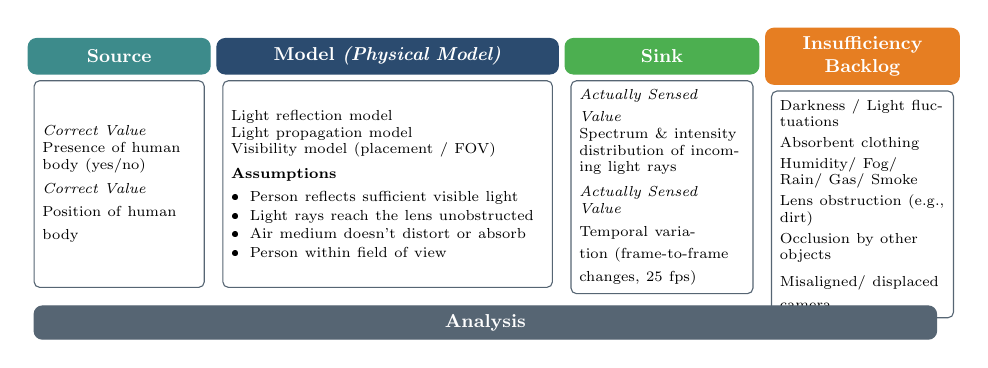
\begin{tikzpicture}[scale=0.75, transform shape, node distance=0.15cm]

    % Headers
    \node[rcsbox=rcsteal, text width=2.8cm, minimum height=0.6cm] (source-h) {Source};
    \node[rcsbox=rcsblue, text width=5.5cm, minimum height=0.6cm, right=0.1cm of source-h] (model-h) {Model \textit{(Physical Model)}};
    \node[rcsbox=rcsgreen, text width=3cm, minimum height=0.6cm, right=0.1cm of model-h] (sink-h) {Sink};
    \node[rcsbox=rcsorange, text width=3cm, minimum height=0.6cm, right=0.1cm of sink-h] (backlog-h) {Insufficiency Backlog};

    % Source content
    \node[rcsoutline, text width=2.6cm, below=0.1cm of source-h, align=left, inner sep=4pt, minimum height=3.5cm] (source-c) {
        \textit{\scriptsize Correct Value}\\
        \scriptsize Presence of human body (yes/no)\\[4pt]
        \textit{\scriptsize Correct Value}\\
        \scriptsize Position of human body
    };

    % Model content
    \node[rcsoutline, text width=5.3cm, below=0.1cm of model-h, align=left, inner sep=4pt, minimum height=3.5cm] (model-c) {
        \scriptsize Light reflection model\\
        \scriptsize Light propagation model\\
        \scriptsize Visibility model (placement / FOV)\\[4pt]
        \textbf{\scriptsize Assumptions}\\
        \begin{itemize}[leftmargin=*, itemsep=1pt, parsep=0pt, topsep=1pt, font=\scriptsize]
            \item Person reflects sufficient visible light
            \item Light rays reach the lens unobstructed
            \item Air medium doesn't distort or absorb
            \item Person within field of view
        \end{itemize}
    };

    % Sink content
    \node[rcsoutline, text width=2.8cm, below=0.1cm of sink-h, align=left, inner sep=4pt, minimum height=3.5cm] (sink-c) {
        \textit{\scriptsize Actually Sensed Value}\\
        \scriptsize Spectrum \& intensity distribution of incoming light rays\\[4pt]
        \textit{\scriptsize Actually Sensed Value}\\
        \scriptsize Temporal variation (frame-to-frame changes, 25 fps)
    };

    % Backlog content
    \node[rcsoutline, text width=2.8cm, below=0.1cm of backlog-h, align=left, inner sep=4pt, minimum height=3.5cm] (backlog-c) {
        \scriptsize Darkness / Light fluctuations\\[2pt]
        \scriptsize Absorbent clothing\\[2pt]
        \scriptsize Humidity/ Fog/ Rain/ Gas/ Smoke\\[2pt]
        \scriptsize Lens obstruction (e.g., dirt)\\[2pt]
        \scriptsize Occlusion by other objects\\[2pt]
        \scriptsize Misaligned/ displaced camera
    };

    % Analysis section
    \node[rcsbox=rcsgray, text width=15cm, minimum height=0.5cm, below=0.3cm of source-c.south west, anchor=north west] (analysis-h) {Analysis};

\end{tikzpicture}
\caption{Appendix Figure 2: C -> A Analysis}
\label{fig:c-to-a}
\end{figure}

\newpage

%% Appendix Figure 4: C -> A Traceability Matrix
\begin{landscape}
\begin{table}[H]
\centering
\caption{Appendix Figure 4: C -> A Traceability Matrix}
\label{tab:c-a-matrix}
\tiny
\setlength{\tabcolsep}{2pt}
\begin{tabular}{|p{0.8cm}|p{2cm}|p{2.5cm}|p{2.5cm}|p{2.5cm}|p{2.5cm}|p{2.5cm}|p{2.5cm}|}
\hline
\rowcolor{rcslightgray}
& \textbf{Failure Modes} & \textbf{FM\textsubscript{1}} & \textbf{FM\textsubscript{2}} & \textbf{FM\textsubscript{3}} & \textbf{FM\textsubscript{4}} & \textbf{FM\textsubscript{5}} & \textbf{FM\textsubscript{6}} \\
\hline
\rowcolor{rcslightgray}
\textbf{Assumptions} & & Timing Late & Timing Early & Provision Commission & Provision Omission & Data Subtle & Data Coarse \\
\hline
\cellcolor{rcsblue!20}\textbf{A\textsubscript{1}} & Person reflects sufficient visible light &
\cellcolor{rcsgreen!20}TC\textsubscript{11}: Person steps from darkness into light &
\cellcolor{rcsteal!20}TC\textsubscript{12}: Sudden glare or specular reflection before person enters area &
\cellcolor{rcsorange!20}TC\textsubscript{13}: Highly reflective background objects (= person-like features) &
\cellcolor{rcsyellow!20}TC\textsubscript{14}: Person wearing dark, non-reflective clothing (absorbent material) &
\cellcolor{rcslightblue!20}TC\textsubscript{15}: Low reflectance clothing and low ambient light/ darkness &
\cellcolor{rcsred!20}TC\textsubscript{16}: Overexposure / bloom (strong direct light) saturates pixels \\
\hline
\cellcolor{rcsblue!20}\textbf{A\textsubscript{2}} & Medium doesn't distort or absorb &
\cellcolor{rcsgreen!20}TC\textsubscript{21}: Fog or steam dissipates just before detection &
\cellcolor{rcsteal!20}TC\textsubscript{22}: Rain or water distortion leads to illusion of smaller distance &
\cellcolor{rcsorange!20}TC\textsubscript{23}: Dense rain droplets produce bright/dark patterns that mimic person &
\cellcolor{rcsyellow!20}TC\textsubscript{24}: Thick fog or heavy rain attenuates person signature &
\cellcolor{rcslightblue!20}TC\textsubscript{25}: Light haze or high humidity blurs edges and reduces contrast &
\cellcolor{rcsred!20}TC\textsubscript{26}: Dense dust/ smoke creates large textured blobs \& coarse shapes \\
\hline
\cellcolor{rcsblue!20}\textbf{A\textsubscript{3}} & Light rays reach the lens unobstructed &
\cellcolor{rcsgreen!20}TC\textsubscript{31}: Temporary occlusion enters frame, delaying person detection &
\cellcolor{rcsteal!20}TC\textsubscript{32}: Passing occlusion classified as person &
\cellcolor{rcsorange!20}TC\textsubscript{33}: Transient reflections create person-like contours &
\cellcolor{rcsyellow!20}TC\textsubscript{34}: Obstruction of lens causes reduced or no feature visibility &
\cellcolor{rcslightblue!20}TC\textsubscript{35}: Thin film causes subtle blurring of person edges &
\cellcolor{rcsred!20}TC\textsubscript{36}: Lens heavily occluded/scratched; image shows large indistinct regions \\
\hline
\cellcolor{rcsblue!20}\textbf{A\textsubscript{4}} & Person within field of view &
\cellcolor{rcsgreen!20}TC\textsubscript{41}: Person enters the peripheral FOV first, only later moves into central detection zone &
\cellcolor{rcsteal!20}TC\textsubscript{42}: Person silhouette appears momentarily at the edge, triggering detection early &
\cellcolor{rcsorange!20}TC\textsubscript{43}: Background object with human-like vertical shape at the edge of FOV &
\cellcolor{rcsyellow!20}TC\textsubscript{44}: Camera is misaligned or displaced &
\cellcolor{rcslightblue!20}TC\textsubscript{45}: Person partially occluded by scene elements, only subtle features visible &
\cellcolor{rcsred!20}TC\textsubscript{46}: Person at extreme distance with low pixel footprint \\
\hline
\end{tabular}
\end{table}
\end{landscape}

\newpage

%% Appendix Figure 3: A -> R
\begin{figure}[H]
\centering
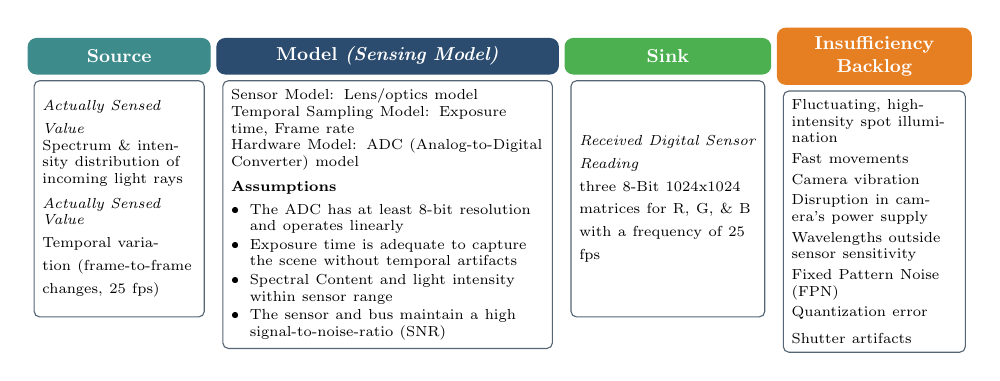
\begin{tikzpicture}[scale=0.75, transform shape, node distance=0.15cm]

    % Headers
    \node[rcsbox=rcsteal, text width=2.8cm, minimum height=0.6cm] (source-h) {Source};
    \node[rcsbox=rcsblue, text width=5.5cm, minimum height=0.6cm, right=0.1cm of source-h] (model-h) {Model \textit{(Sensing Model)}};
    \node[rcsbox=rcsgreen, text width=3.2cm, minimum height=0.6cm, right=0.1cm of model-h] (sink-h) {Sink};
    \node[rcsbox=rcsorange, text width=3cm, minimum height=0.6cm, right=0.1cm of sink-h] (backlog-h) {Insufficiency Backlog};

    % Source content
    \node[rcsoutline, text width=2.6cm, below=0.1cm of source-h, align=left, inner sep=4pt, minimum height=4cm] (source-c) {
        \textit{\scriptsize Actually Sensed Value}\\
        \scriptsize Spectrum \& intensity distribution of incoming light rays\\[4pt]
        \textit{\scriptsize Actually Sensed Value}\\
        \scriptsize Temporal variation (frame-to-frame changes, 25 fps)
    };

    % Model content
    \node[rcsoutline, text width=5.3cm, below=0.1cm of model-h, align=left, inner sep=4pt, minimum height=4cm] (model-c) {
        \scriptsize Sensor Model: Lens/optics model\\
        \scriptsize Temporal Sampling Model: Exposure time, Frame rate\\
        \scriptsize Hardware Model: ADC (Analog-to-Digital Converter) model\\[4pt]
        \textbf{\scriptsize Assumptions}\\
        \begin{itemize}[leftmargin=*, itemsep=1pt, parsep=0pt, topsep=1pt, font=\scriptsize]
            \item The ADC has at least 8-bit resolution and operates linearly
            \item Exposure time is adequate to capture the scene without temporal artifacts
            \item Spectral Content and light intensity within sensor range
            \item The sensor and bus maintain a high signal-to-noise-ratio (SNR)
        \end{itemize}
    };

    % Sink content
    \node[rcsoutline, text width=3cm, below=0.1cm of sink-h, align=left, inner sep=4pt, minimum height=4cm] (sink-c) {
        \textit{\scriptsize Received Digital Sensor Reading}\\
        \scriptsize three 8-Bit 1024x1024 matrices for R, G, \& B with a frequency of 25 fps
    };

    % Backlog content
    \node[rcsoutline, text width=2.8cm, below=0.1cm of backlog-h, align=left, inner sep=4pt, minimum height=4cm] (backlog-c) {
        \scriptsize Fluctuating, high-intensity spot illumination\\[2pt]
        \scriptsize Fast movements\\[2pt]
        \scriptsize Camera vibration\\[2pt]
        \scriptsize Disruption in camera's power supply\\[2pt]
        \scriptsize Wavelengths outside sensor sensitivity\\[2pt]
        \scriptsize Fixed Pattern Noise (FPN)\\[2pt]
        \scriptsize Quantization error\\[2pt]
        \scriptsize Shutter artifacts
    };

\end{tikzpicture}
\caption{Appendix Figure 3: A -> R Analysis}
\label{fig:a-to-r}
\end{figure}

%% A -> R Traceability Matrix
\begin{landscape}
\begin{table}[H]
\centering
\caption{A -> R Traceability Matrix}
\label{tab:a-r-matrix}
\tiny
\setlength{\tabcolsep}{2pt}
\begin{tabular}{|p{0.8cm}|p{2.2cm}|p{2.5cm}|p{2.5cm}|p{2.5cm}|p{2.5cm}|p{2.5cm}|p{2.5cm}|}
\hline
\rowcolor{rcslightgray}
& \textbf{Failure Modes} & \textbf{FM\textsubscript{1}} & \textbf{FM\textsubscript{2}} & \textbf{FM\textsubscript{3}} & \textbf{FM\textsubscript{4}} & \textbf{FM\textsubscript{5}} & \textbf{FM\textsubscript{6}} \\
\hline
\rowcolor{rcslightgray}
\textbf{Assumptions} & & Timing Late & Timing Early & Provision Commission & Provision Omission & Data Subtle & Data Coarse \\
\hline
\cellcolor{rcsblue!20}\textbf{A\textsubscript{1}} & ADC has 8-bit resolution and operates linearly &
TC\textsubscript{11}: ADC auto-exposure + 8-bit quantization requires multiple frames to settle &
TC\textsubscript{12}: Quantization step noise or transient peak in a single frame &
TC\textsubscript{13}: Quantization artifacts or banding produce person-like edges/patterns &
TC\textsubscript{14}: 8-bit saturation removes subtle gradients that indicate a person &
TC\textsubscript{15}: Low bit depth causes low contrast for small/remote person pixels &
TC\textsubscript{16}: Severe quantization + dithering produces blocky/coarse pixel patterns \\
\hline
\cellcolor{rcsblue!20}\textbf{A\textsubscript{2}} & Exposure time is adequate to capture scene without temporal artifacts &
TC\textsubscript{21}: Readout hiccup / frame drop occurs during approach &
TC\textsubscript{22}: Frame duplication/ buffer replay presents stale frame &
TC\textsubscript{23}: Jitter in frame timestamp/ corrupted frames produce motion patterns &
TC\textsubscript{24}: High bus contention delays frame read-out, sensor to discards a new frame &
TC\textsubscript{25}: Rolling Shutter Distortion &
TC\textsubscript{26}: Read-out/ process aborted mid-frame due to system error, resulting in partial image frame \\
\hline
\cellcolor{rcsblue!20}\textbf{A\textsubscript{3}} & Spectral Content and light intensity within sensor range &
TC\textsubscript{31}: Sensor requires long exposure time due to low light &
TC\textsubscript{32}: Sensor has insufficient recovery time after severe light saturation &
TC\textsubscript{33}: Specific light wavelength is misinterpreted as a visible object &
TC\textsubscript{34}: Light intensity is too low to detect a person's presence. &
TC\textsubscript{35}: Scene contrast is lost due to specular reflection &
TC\textsubscript{36}: Extreme low light causes pixel values to be near zero (dark) \\
\hline
\cellcolor{rcsblue!20}\textbf{A\textsubscript{4}} & The sensor and bus maintain a high signal-to-noise-ratio (SNR) &
TC\textsubscript{41}: High SNR maintenance overhead delays the frame read-out &
TC\textsubscript{42}: High thermal noise causes buffer instability, leading to stale data reuse &
TC\textsubscript{43}: Fixed Pattern Noise (FPN) creates false person-like pixel artifacts &
TC\textsubscript{44}: Random noise obscures the subtle edges and features of a person &
TC\textsubscript{45}: High Noise level reduces effective dynamic range of person pixels &
TC\textsubscript{46}: Electrical noise spikes cause individual pixel values to become corrupted \\
\hline
\end{tabular}
\end{table}
\end{landscape}

\newpage

%% R -> E Analysis
\begin{figure}[H]
\centering
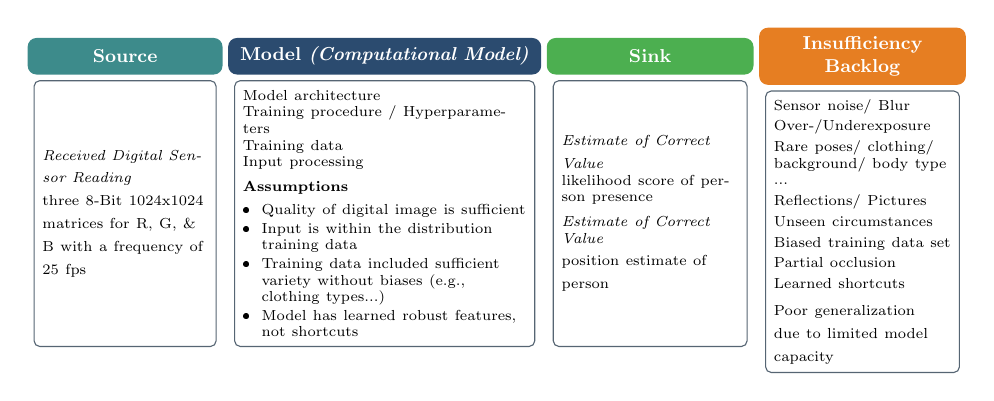
\begin{tikzpicture}[scale=0.75, transform shape, node distance=0.15cm]

    % Headers
    \node[rcsbox=rcsteal, text width=3cm, minimum height=0.6cm] (source-h) {Source};
    \node[rcsbox=rcsblue, text width=5cm, minimum height=0.6cm, right=0.1cm of source-h] (model-h) {Model \textit{(Computational Model)}};
    \node[rcsbox=rcsgreen, text width=3.2cm, minimum height=0.6cm, right=0.1cm of model-h] (sink-h) {Sink};
    \node[rcsbox=rcsorange, text width=3.2cm, minimum height=0.6cm, right=0.1cm of sink-h] (backlog-h) {Insufficiency Backlog};

    % Source content
    \node[rcsoutline, text width=2.8cm, below=0.1cm of source-h, align=left, inner sep=4pt, minimum height=4.5cm] (source-c) {
        \textit{\scriptsize Received Digital Sensor Reading}\\
        \scriptsize three 8-Bit 1024x1024 matrices for R, G, \& B with a frequency of 25 fps
    };

    % Model content
    \node[rcsoutline, text width=4.8cm, below=0.1cm of model-h, align=left, inner sep=4pt, minimum height=4.5cm] (model-c) {
        \scriptsize Model architecture\\
        \scriptsize Training procedure / Hyperparameters\\
        \scriptsize Training data\\
        \scriptsize Input processing\\[4pt]
        \textbf{\scriptsize Assumptions}\\
        \begin{itemize}[leftmargin=*, itemsep=1pt, parsep=0pt, topsep=1pt, font=\scriptsize]
            \item Quality of digital image is sufficient
            \item Input is within the distribution training data
            \item Training data included sufficient variety without biases (e.g., clothing types...)
            \item Model has learned robust features, not shortcuts
        \end{itemize}
    };

    % Sink content
    \node[rcsoutline, text width=3cm, below=0.1cm of sink-h, align=left, inner sep=4pt, minimum height=4.5cm] (sink-c) {
        \textit{\scriptsize Estimate of Correct Value}\\
        \scriptsize likelihood score of person presence\\[4pt]
        \textit{\scriptsize Estimate of Correct Value}\\
        \scriptsize position estimate of person
    };

    % Backlog content
    \node[rcsoutline, text width=3cm, below=0.1cm of backlog-h, align=left, inner sep=4pt, minimum height=4.5cm] (backlog-c) {
        \scriptsize Sensor noise/ Blur\\[2pt]
        \scriptsize Over-/Underexposure\\[2pt]
        \scriptsize Rare poses/ clothing/ background/ body type ...\\[2pt]
        \scriptsize Reflections/ Pictures\\[2pt]
        \scriptsize Unseen circumstances\\[2pt]
        \scriptsize Biased training data set\\[2pt]
        \scriptsize Partial occlusion\\[2pt]
        \scriptsize Learned shortcuts\\[2pt]
        \scriptsize Poor generalization due to limited model capacity
    };

\end{tikzpicture}
\caption{R -> E Analysis}
\label{fig:r-to-e}
\end{figure}

%% R -> E Traceability Matrix
\begin{landscape}
\begin{table}[H]
\centering
\caption{R -> E Traceability Matrix}
\label{tab:r-e-matrix}
\tiny
\setlength{\tabcolsep}{2pt}
\begin{tabular}{|p{0.8cm}|p{2.2cm}|p{2.5cm}|p{2.5cm}|p{2.5cm}|p{2.5cm}|p{2.5cm}|p{2.5cm}|}
\hline
\rowcolor{rcslightgray}
& \textbf{Failure Modes} & \textbf{FM\textsubscript{1}} & \textbf{FM\textsubscript{2}} & \textbf{FM\textsubscript{3}} & \textbf{FM\textsubscript{4}} & \textbf{FM\textsubscript{5}} & \textbf{FM\textsubscript{6}} \\
\hline
\rowcolor{rcslightgray}
\textbf{Assumptions} & & Timing Late & Timing Early & Provision Commission & Provision Omission & Data Subtle & Data Coarse \\
\hline
\cellcolor{rcsblue!20}\textbf{A\textsubscript{1}} & Quality of digital image is sufficient &
TC\textsubscript{11}: Image sharpness improves only after several frames &
TC\textsubscript{12}: Early frame compression artifact or motion blur &
TC\textsubscript{13}: Noise, blur, or patterns resembling a person &
TC\textsubscript{14}: Image degraded (blur, smear, low resolution) &
TC\textsubscript{15}: Slight motion blur or defocus lowers feature clarity &
TC\textsubscript{16}: Severe compression, low resolution, or defocus \\
\hline
\cellcolor{rcsblue!20}\textbf{A\textsubscript{2}} & Input is within the distribution training data &
TC\textsubscript{21}: Out-of-distribution (OOD) scene causes model to hesitate &
TC\textsubscript{22}: OOD feature triggers early false activation &
TC\textsubscript{23}: Objects seen in training (e.g., mannequins, shadows) resemble humans &
TC\textsubscript{24}: Person outside training distribution (e.g., unusual clothing/ posture) &
TC\textsubscript{25}: Slight distribution shift (e.g., new camera angle, illumination, fisheye lens) &
TC\textsubscript{26}: Strong distribution shift (e.g., infrared illumination, fisheye lens) \\
\hline
\cellcolor{rcsblue!20}\textbf{A\textsubscript{3}} & Training data included sufficient variety without biases &
TC\textsubscript{31}: Under-represented groups (e.g., specific clothing colors) &
TC\textsubscript{32}: Model over-fits to one feature, detects object with shared feature &
TC\textsubscript{33}: Shortcut in training, causing mis-identification of background &
TC\textsubscript{34}: Under-represented demographics/ poses not recognized &
TC\textsubscript{35}: Features for a particular subgroup captured poorly &
TC\textsubscript{36}: Model generalizes poorly to certain body types or apparel \\
\hline
\cellcolor{rcsblue!20}\textbf{A\textsubscript{4}} & Model has learned robust features, not shortcuts &
TC\textsubscript{41}: Model depends on context features (e.g., shadows) &
TC\textsubscript{42}: Shortcut cue appears early &
TC\textsubscript{43}: Shortcut feature in background wrongly activates &
TC\textsubscript{44}: Shortcut fails, so the person is not detected &
TC\textsubscript{45}: Shortcut cue is partially present, model confidence fluctuates &
TC\textsubscript{46}: Shortcut-based model generalizes poorly \\
\hline
\end{tabular}
\end{table}
\end{landscape}

\end{document}
